\documentclass[12pt,a4paper]{article}
\usepackage{graphicx} 

\renewcommand{\familydefault}{\sfdefault}
\usepackage{helvet}

\usepackage[T1]{fontenc}
\usepackage{inconsolata}

\newcommand{\inlinecode}{\texttt}
\usepackage{hyperref}

\title{CrapStore}
\author{Niels de Bruin\\
	Georgios Andreadis}
\date{January - April 2016}

\begin{document}

%\maketitle
\begin{titlepage}
	\centering
	\vfill
	{\bfseries\LARGE
		CrapStore
	}
	\vskip2cm
	{\bfseries
		Niels de Bruin\\
		Georgios Andreadis\\
	} 
	\vfill
	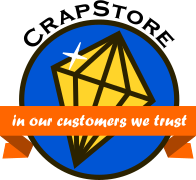
\includegraphics[width=4cm]{../client/images/logo_large.png}
	\vfill
	\vfill
\end{titlepage}
\pagebreak

\tableofcontents
\pagebreak

%%%%%%%%%%%%%%%%%%%%%%%%%%%%%%%%%%%%%%%%%%%%%%%%%%%%%%%%%%%%%%%%%%%
\section{Introduction}
Have you ever tried to hack into an application that you have built? If you haven't yet, or if you just like breaking things, CrapStore is the tool for you.

% % % % % % % % % % % % % % % % % % % % % % % % % % % % % % % % % %
\subsection{What is CrapStore?}
In a nutshell, CrapStore is a modern version of BadStore, a penetration testing practice tool for web developers. In other words, it is a webshop full of security flaws and vulnerabilities, waiting for you to find and exploit them. In contrast to the original BadStore platform, CrapStore is built on top of the (more up-to-date) node.js JavaScript server platform.

We are not affiliated with the BadStore project in any way, but the list of exploits and the contents of this webshop were primarily inspired by the BadStore application.

% % % % % % % % % % % % % % % % % % % % % % % % % % % % % % % % % %
\subsection{The Purpose of CrapStore}
By exploring the various vulnerabilities modern web systems have to offer, you look at web applications from the point of view of a hacker - somebody who wants to penetrate a system. This can be a valuable insight, because instead of trying to make things work, you are trying to break the application on purpose. It is our hope that you can learn from this experience and, as a result, can increase the security of your own site.

The vulnerabilities you can find in CrapStore are not purely fictional - they are (unfortunately) far more common than you might think. This is why CrapStore can help make you aware of what can go wrong, so that you can fill up the loopholes in time, before someone else sneaks through them.

% % % % % % % % % % % % % % % % % % % % % % % % % % % % % % % % % %
\section{Disclaimer}
To be clear: this is \emph{not} a safe web application. Don't enter sensitive information! And, perhaps more importantly, don't expect us to send you a real iPad.

Perform these penetration tests on websites only if you have the written consent of their owners to do so, and even then perform them in a secured offline environment. Try these attacks at your own risk, we assume no responsibility at all for any and all possible damage caused.

%%%%%%%%%%%%%%%%%%%%%%%%%%%%%%%%%%%%%%%%%%%%%%%%%%%%%%%%%%%%%%%%%%%
\section{Installation}
To setup the MySQL database instance, run \inlinecode{schema.sql} and \inlinecode{sample.sql} (as well as any time you want a fresh install of the database). All required NPM packages are listed in the \inlinecode{package.json} file. That just leaves you to run \inlinecode{npm install}, which installs all necessary packages. Then, \inlinecode{bower install} will download and insert the necessary dependencies into the project (such as jQuery or Bootstrap).

This is a grunt-based project, thus executing the 'serve' task of grunt (by executing \inlinecode{grunt serve}) starts the server on \url{http://localhost:1337}.


%%%%%%%%%%%%%%%%%%%%%%%%%%%%%%%%%%%%%%%%%%%%%%%%%%%%%%%%%%%%%%%%%%%
\section{Exploits}
As previously stated, this list is \emph{strongly} inspired by BadStore. Only some of the exploits from that list have been removed, due to them being less relevant or likely to occur in the modern context.

% % % % % % % % % % % % % % % % % % % % % % % % % % % % % % % % % %
\subsection{Authentication}
\subsubsection{Weak Password Recovery System}
\paragraph{Where?}
The 'forgot password' page and the registration page

\paragraph{What?}
Having a single, uniform recovery question with a very limited set of possible answers might not be the best idea from a security perspective. Try user names from the guest book and see if you can hack into an account.

\subsubsection{Unprotected admin page}
\paragraph{Where?}
Figure this one out for yourself

\paragraph{What?}
There are some admin operations possible for non-admin users that should not be possible.

\subsubsection{Brute-force Password Attack}
\paragraph{Where?}
The login page

\paragraph{What?}
Try some account emails from the guest book and do a brute force attack with simple passwords. Once inside (with the right user credentials), maybe have a look at the supplier portal? One particular supplier is our main source of products, and he even exposes his email address in the guest book!

\subsubsection{Supplier portal}
\paragraph{Where?}
Guest book and login page

\paragraph{What?}
Try to log in as a supplier and see if you can break our image upload and all kinds of stuff in the product info category!

% % % % % % % % % % % % % % % % % % % % % % % % % % % % % % % % % %
\subsection{Authorization}
\subsubsection{Session prediction}
\paragraph{Where?}
The entire site

\paragraph{What?}
Alarm bells should be ringing in your head when you look at the session IDs generated by this site.

\subsubsection{Insufficient Session Expiration}
\paragraph{Where?}
The entire site

\paragraph{What?}
Hint: Session IDs only expire only on one side.

% % % % % % % % % % % % % % % % % % % % % % % % % % % % % % % % % %
\subsection{Cross-Site Scripting}
\paragraph{Where?}
The guest book and the supplier portal

\paragraph{What?}
Hint: inputs to the submit forms are (unfortunately for us, or fortunately for you) not escaped.

% % % % % % % % % % % % % % % % % % % % % % % % % % % % % % % % % %
\subsection{SQL Injection}
\paragraph{Where?}
Search box on the product page

\paragraph{What?}
Try manipulating the query and see if you can uncover some secret, limited edition products.

% % % % % % % % % % % % % % % % % % % % % % % % % % % % % % % % % %
\subsection{Cookie Manipulation}
\paragraph{Where?}
The entire page

\paragraph{What?}
Add some products to the cart, and have a look at the cookies. Do you notice something that could be used to your advantage (and the stores disadvantage)?

\end{document}